% cls && pdflatex lab-5-report.tex && cls && pdflatex lab-5-report.tex && start lab-5-report.pdf
\documentclass[12pt, a4paper]{article}
\usepackage[T2A]{fontenc}
\usepackage[utf8]{inputenc}
\usepackage[english,ukrainian]{babel}
\usepackage{amsmath, amssymb}
\usepackage{verbatim}

\usepackage[top = 2 cm, left = 1 cm, right = 1 cm, bottom = 2 cm]{geometry}

\usepackage{float, graphicx}
\usepackage{amsthm}
\newtheorem{lemma}{Лема}
\newtheorem*{lemma*}{Лема}
\newtheorem{theorem}{Теорема}
\newtheorem*{theorem*}{Теорема}
\newtheorem{definition}{Визначення}
\newtheorem*{definition*}{Визначення}
\theoremstyle{definition}
\newtheorem{remark}{Зауваження}
\newtheorem*{remark*}{Зауваження}
\newtheorem{example}{Приклад}
\newtheorem*{example*}{Приклад}
\newtheorem{problem}{Задача}
\newtheorem*{problem*}{Задача}
\newtheorem{solution}{Розв'язок}
\newtheorem*{solution*}{Розв'язок}
\newtheorem{corollary}{Наслідок}
\newtheorem*{corollary*}{Наслідок}

\newcommand{\NN}{\mathbb{N}}
\newcommand{\RR}{\mathbb{R}}
\newcommand{\CC}{\mathbb{C}}
\newcommand{\HH}{\mathcal{H}}
\newcommand{\Min}{\displaystyle\min\limits}
\newcommand{\Max}{\displaystyle\max\limits}
\newcommand{\Sup}{\displaystyle\sup\limits}
\newcommand{\Sum}{\displaystyle\sum\limits}
\newcommand{\Prod}{\displaystyle\prod\limits}
\newcommand{\Int}{\displaystyle\int\limits}
\newcommand{\Iint}{\displaystyle\iint\limits}
\newcommand{\Lim}{\displaystyle\lim\limits}

\newcommand*\diff{\mathop{}\!\mathrm{d}}

\renewcommand{\bf}[1]{\textbf{#1}}
\renewcommand{\epsilon}{\varepsilon}
\renewcommand{\phi}{\varphi}

\DeclareMathOperator{\signum}{sign}
\DeclareMathOperator{\diam}{diam}
\DeclareMathOperator{\rang}{rang}
\DeclareMathOperator{\const}{const}
\DeclareMathOperator{\cond}{cond}
\DeclareMathOperator{\diagonal}{diag}

\numberwithin{equation}{section}

\setlength\parindent{0pt}
\allowdisplaybreaks

\newcommand{\cover}[2]{
\begin{center}
\hfill \break
	Міністерство освіти та науки України \\
	Київський національний університет імені Тараса Шевченка \\ 
	Факультет комп'ютерних наук та кібернетики \\
	Кафедра обчислювальної математики
\end{center}

\vfill 

\begin{center}
	\large{
		Звіт до лабораторної роботи №{#1} на тему: \\ 
		``{#2}''
	}
\end{center}

\vfill 

\begin{flushright}
	Виконав студент групи ОМ-3 \\
	Скибицький Нікіта
\end{flushright}

\vfill 

\begin{center}
    Київ, 2018 
\end{center}

\thispagestyle{empty} 
\newpage
}

\begin{document}

\cover{5}{Найкраще середньоквадратичне наближення}

% \tableofcontents

\section{Постановка задачі}

Усі завдання будуть виконані для функції $f$ вигляду: \[ f(x) = \frac{|x - 4| + |x + 4|}{2}, \quad a = -10 \le x \le 10 = b. \] Також задамо $n = 4$, $m = 20$. У всіх підзадачах необхідно побудувати графіки функцій $f(x)$ та отриманого наближення, обчислити відхилення.

\subsection{Найкраще середньоквадратичне наближення}

Побудувати поліном найкращого середньоквадратичного наближення $Q_n(x)$ для функції $f(x)$ на проміжку $[a, b]$, вибравши в якості лінійно незалежних функцій систему функцій $\phi_i(x)$, для $i=\overline{0,n}$. Системи функцій які будуть розглянуті:
\begin{enumerate}
    % \item $\phi_i(x) = x^i$;
    \item $\phi_i(x) = T_i(x)$;
    % \item експоненційна;
    \item тригонометрична.
\end{enumerate}

\subsection{Метод найменших квадратів}

Функція $y = f(x)$ задана таблицею значень $y_0, y_1, \ldots, y_m$ у точках $x_0, x_1, \ldots, x_m$. Використовуючи метод найменших квадратів (МНК), знайти поліном $Q_n(x) = a_0 + a_1 \cdot x + \ldots + a_n \cdot x^n$ найкращого середньоквадратичного наближення оптимального степеня $n = n^\star$. За оптимальне значення $n^\star$ будемо вважати той степінь поліному, починаючи з якого величина \[ \sigma_n = \sqrt{\frac{1}{m - n} \cdot \sum_{k = 0}^m (Q_n(x_k)^2 - y_k)^2} \] стабілізується або починає зростати.

\subsection{Кубічні згладжувальні сплайни}

Побудувати кубічний згладжувальний  сплайн для функції $f(x)$ на проміжку $[a, b]$ за її значеннями у вузлах $x_i = a + i \cdot h$, для $i = \overline{0, m}$, де $h = (b - a) / m$, а $m \gg n$.

\section{Теоретична частина}

\subsection{Найкраще середньоквадратичне наближення}

Наблизимо функцію $f: \HH \to \RR$ з гільбертового простору $\HH$ функціями зі скінченновимірного підпростору $M_n$ простору $\HH$. Скалярний добуток у просторі $\HH$ ми будемо позначати як $(u, v)$, відповідну норму -- як $\|u\| = \sqrt{(u, u)}$. \\

Нехай $\{\phi_i\}_{i=0}^\infty$ -- лінійно-незалежна система функцій $\HH \to \RR$. Розглянемо її скінченну підсистему $\{\phi_i\}_{i=0}^n$. Позначимо лінійну оболонку цієї підсистеми за $M_n \subset \HH$. \\

Нагадаємо визначення ЕНН $\Phi$: \[ \|f - \Phi\| = \sqrt{(f - \Phi, f - \Phi)} = \inf_{\phi \in M_n} \|f - \phi\|. \] Якщо $\Phi$ -- ЕНН, то $(f - \Phi, \phi) = 0$ для довільного $\phi \in M_n$, тому можна записати $f = \Phi + \psi$, де $\Phi \in M_n$, $\psi \in M_n^\perp$, тому будемо шукати наближення у вигляді \[ \Phi = \sum_{i = 0}^n c_i \cdot \phi_i. \]

Для виконання $(f - \Phi, \phi) = 0$ достатньо, щоб \[ (f - \Phi, \phi_j) = 0, \quad j = \overline{0, n}, \] що у свою чергу дає \[ \left(f - \sum_{i = 0}^n c_i \cdot \phi_i, \phi_j \right) = 0, \quad j = \overline{0, n}. \] Звідси маємо СЛАР на $c_i$: \[ \sum_{i=0}^n c_i \cdot (\phi_i, \phi_j) = (f, \phi_j), \quad j = \overline{0, n}. \]

Матриця цієї СЛАР -- $G = \|g_{ij}\|_{i,j=1}^{n}$, де $g_{ij} = (\phi_i, \phi_j)$ -- матриця Грамма лінійно-незалежної системи функцій $\{\phi_i\}_{i=0}^n$, що доводить існування та єдиність ЕНН. Оскільки $G^T = G$, то для розв'язування цієї СЛАР використовують метод квадратних коренів. У багатьох випадках матриця $G$ погано обумовлена, у цих випадках систему функцій ортонормують, тобто досягають того, щоб $(\phi_i, \phi_j) = \delta_{ij}$. \\

Явно запишемо розв'язок СЛАР: \[ \Phi = \sum_{i = 0}^n (f, \phi_i) \cdot \phi_i, \] звідки у випадку ортонормованої системи функцій маємо наступний вираз відхилення: \[ \Delta^2(f) = \|f - \Phi\|^2 = \|f\| - \|\Phi\|^2 = \|f\| - \sum_{i=0}^n c_i^2.\] У випадку ортогональної але не нормалізованої системи відхилення шукається наступним чином: \[ \Delta^2(f) = \|f - \Phi\|^2 = \|f\| - \|\Phi\|^2 = \|f\| - \sum_{i=0}^n c_i^2 \cdot \|\phi_i\|^2.\]

\subsection{Метод найменших квадратів}

Нехай в результаті вимірювань функції $f(x)$ маємо таблицю значень: \[ y_i \approx f(x_i), \quad x_i \in [a, b], \quad i = \overline{0, m}.\] За даними цієї таблиці треба побудувати аналітичну формулу $\Phi(x; a_1, a_2, \ldots, a_n)$ таку, що \[ \phi(x_i; a_1, a_2, \ldots, a_n) \approx y_i, \quad i = \overline{0, m}.\] 

Розв'язувати цю задачу інтерполюванням (тобто задавати ``$=$'' замість ``$\approx$'') не раціонально, адже $m \gg n$ і отримана система буде перевизначена, її розв'язки як правило не існують. \\

Параметри $a_1, a_2, \ldots, a_n$ визначають з міркувань \[I(a_1, a_2, \ldots, a_n) = \sum_{i = 0}^m (y_i - \phi(x_i; a_1, a_2, \ldots, a_n)^2 \to \min,\] тому метод і називається методом найменших (суми) квадратів (відхилень). \\

Для досягнення мінімуму достатньо $\partial I / \partial a_i = 0$, для $i = \overline{0, n}$. Зокрема, якщо $\phi$ лінійно залежить від параметрів $a_1, a_2, \ldots, a_n$, то отримаємо СЛАР \[ \sum_{j = 0}^n a_j \cdot \phi_j(x_i) = y_i, \quad i = \overline{0, m},\] яку називають системою умовних рівнянь. \\

МНК рівносильний знаходженню ЕНН у гільбертовому просторі функцій $f: X \to \RR$ над дискретною множиною $X = \{x_0, x_1, \ldots, x_m\}$, у якому скалярний добуток визначається наступним чином: \[ (u, v) = \sum_{i = 0}^m u(x_i) \cdot v(x_i). \] Якщо відомі оцінки похибок $\epsilon_i$ для значень $y_i$ то скалярний добуток задають у вигляді \[ (u, v) = \sum_{i = 0}^m \frac{u(x_i) \cdot v(x_i)}{\epsilon_i^2}. \]

\subsection{Кубічні згладжувальні сплайни}

Нехай деяка функція $f(x)$ задана на відрізку $[a, b]$, що розбитий на сегменти $[x_i, x_{i + 1}]$. Природнім кубічним сплайном називається функція $S(x)$ така, що:
\begin{enumerate}
    \item на кожному відрізку $[x_i, x_{i + 1}]$ є поліномом степеню не вище третього;
    \item має неперервні першу і другу похідну на усьому $[a, b]$;
    \item у точках $x_i$ виконується $S(x_i) = f(x_i)$, тобто сплайн $S$ інтерполює функцію $f$ у точках $x_i$;
    \item $S''(a) = S''(b) = 0$, умова природності.
\end{enumerate}

Побудуємо природній сплайн. З перших двох умов: \[ S''(x) = m_i \cdot \frac{x_{i + 1} - x}{h_i} + m_{i + 1} \cdot \frac{x - x_i}{h_i}; \quad m_i = S''(x_i), \quad h_i = x_{i + 1} - x_i. \] 

Двічі інтегруючи це співвідношення знаходимо: \[ S(x) = m_i \cdot \frac{(x_{i + 1} - x)^3}{6 h_i} + m_{i + 1} \cdot \frac{(x - x_i)^3}{6 h_i} + A_i \cdot \frac{x_{i + 1} - x}{h_i} + B_i \cdot \frac{x - x_i}{h_i}. \] 

Константи $A_i, B_i$ можна знайти з умов $S(x_i) = f_i$. Остаточний вигляд кубічного сплайну: \begin{multline*} S(x) = m_i \cdot \frac{(x_{i + 1} - x)^3}{6 h_i} + m_{i + 1} \cdot \frac{(x - x_i)^3}{6 h_i} + \\ + \left( f_i - \frac{m_i \cdot h_i^2}{6} \right) \cdot \frac{x_{i + 1} - x}{h_i} + \left( f_{i + 1} - \frac{m_{i + 1} \cdot h_i^2}{6}\right) \cdot \frac{x - x_i}{h_i}, \quad x \in [x_i, x_{i + 1}], \quad h_i = x_{i + 1} - x_i. \end{multline*}

Причому, враховуючи, що $S'(x_i - 0) = S'(x_i + 0)$ і умову природності, отримаємо СЛАР для знаходження всіх $M_i = S''(x_i)$: \[ \left\{ \begin{aligned} & m_0 = 0 \\ & \frac{h_i}{6} \cdot m_{i -1 } + \frac{h_i - h_{i + 1}}{3} \cdot m_i + \frac{h_{i + 1}}{6} \cdot m_{i + 1} = \frac{f_{i + 1} - f_i}{h_{i + 1}} - \frac{f_i - f_{i - 1}}{h_i}, \quad i = \overline{1, n - 1} \\ & m_n = 0. \end{aligned} \right. \]

Ця СЛАР розв'язується методом прогонки адже її матриця три-діагональна.

% мінімізаційні властивості природнього кубічного згладжувального сплайну

\section{Практична частина}

\subsection{Найкраще середньоквадратичне наближення}

% \subsubsection{Степенева система функцій}
% \begin{figure}[H]
%     \centering
%     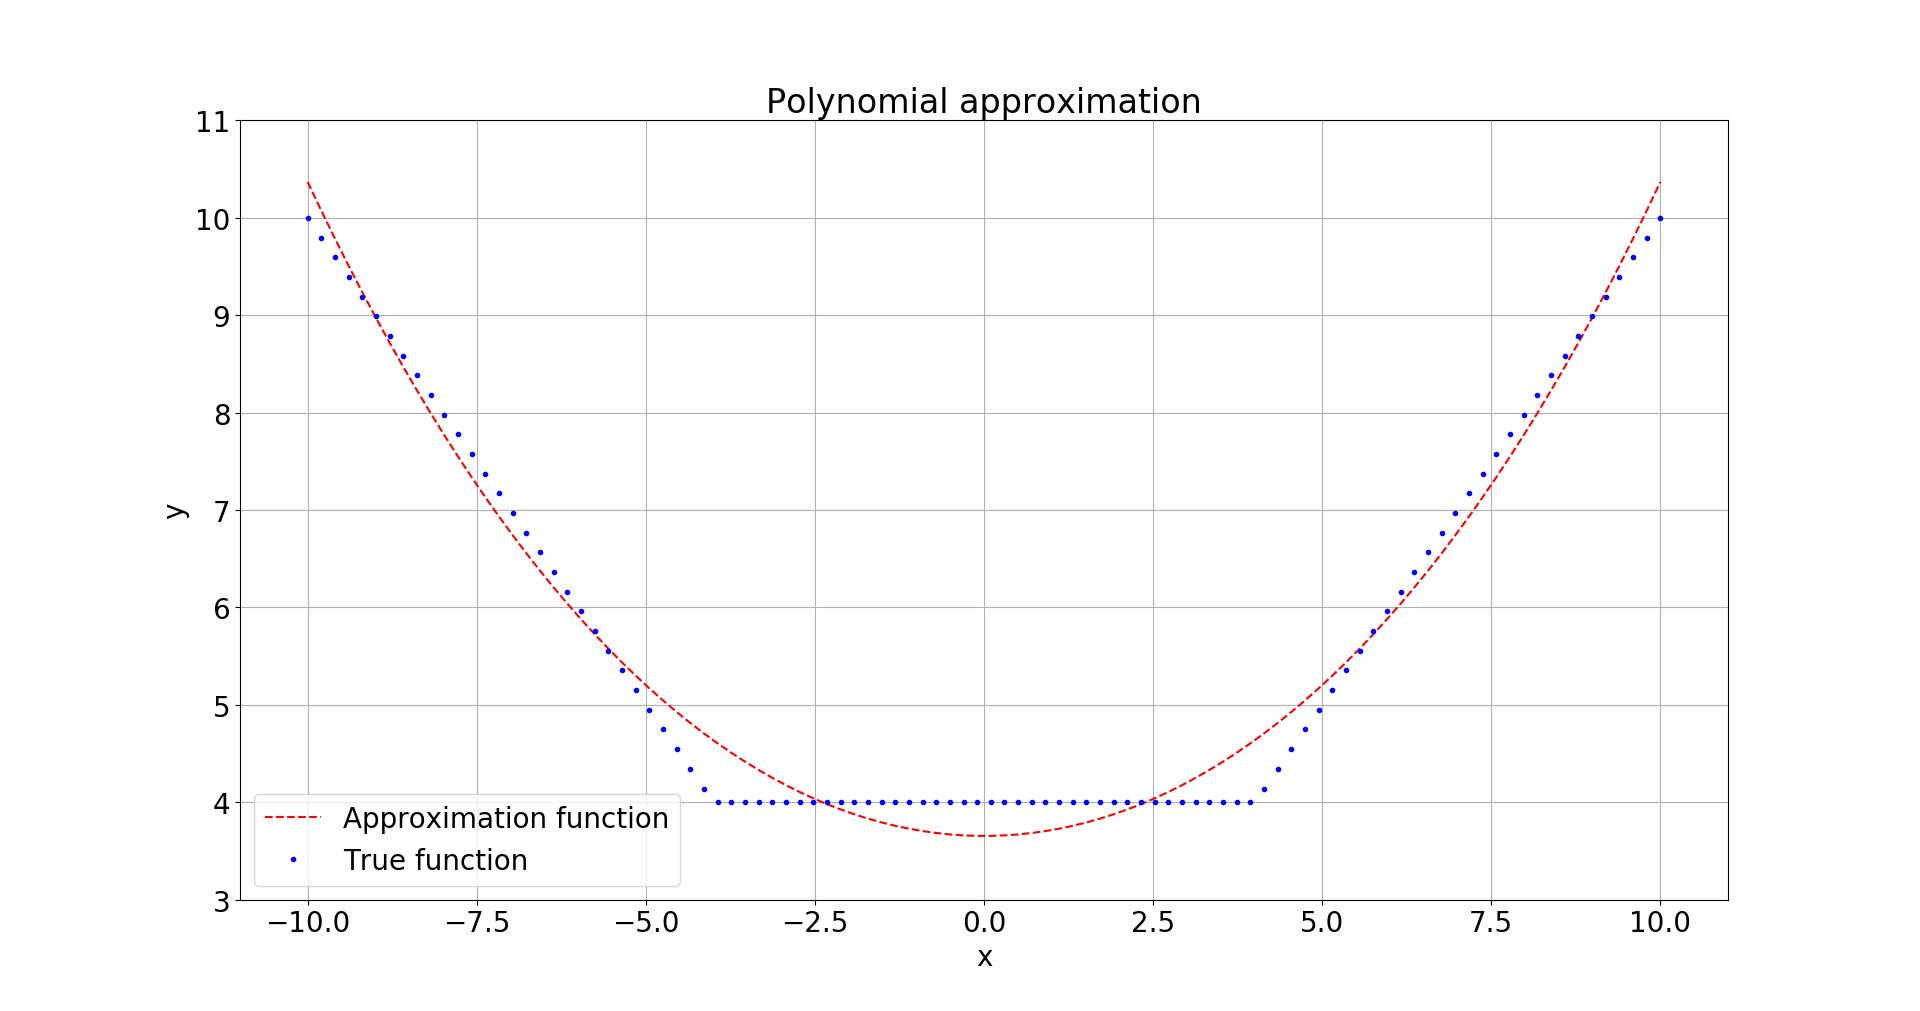
\includegraphics[width=\textwidth]{1.png}
% \end{figure}
% \[ \Delta^2(f) = \texttt{1.3515894719986394}. \]

\subsubsection{Поліноми Чебишева}
\begin{figure}[H]
    \centering
    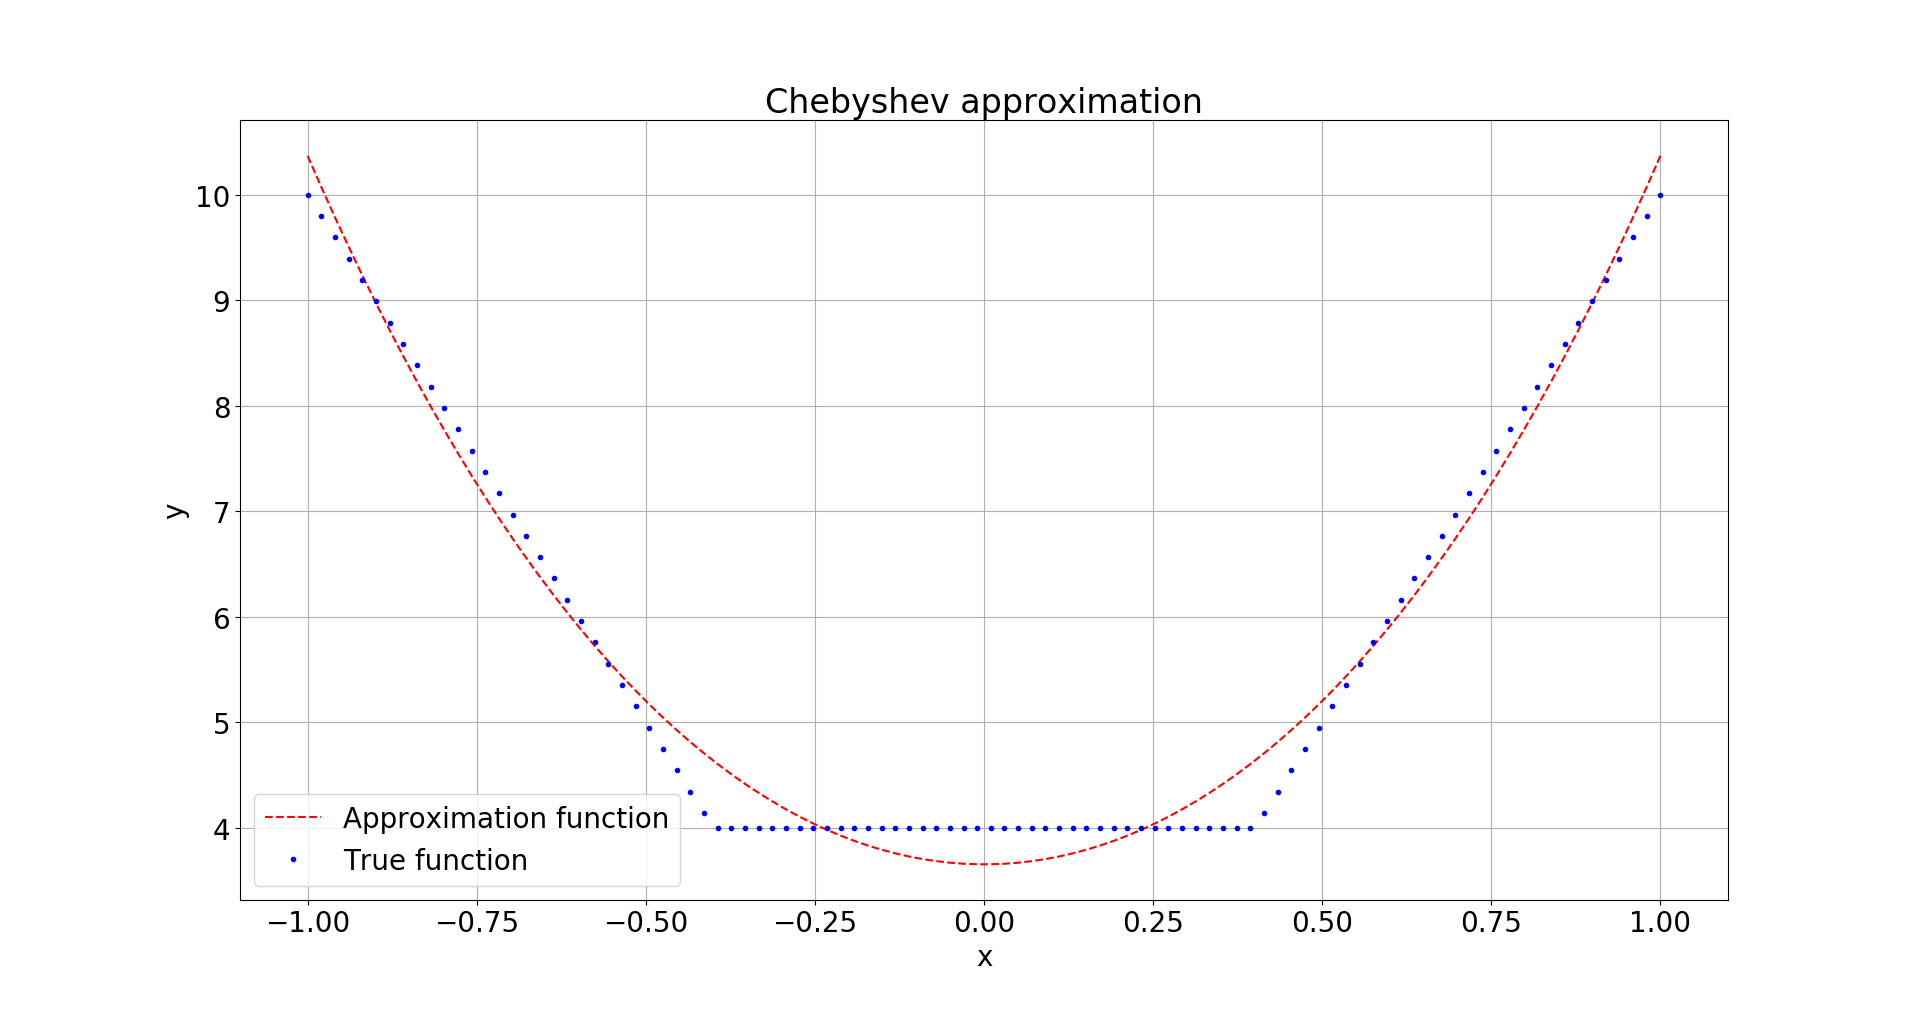
\includegraphics[width=\textwidth]{3.png}
\end{figure}
\[ \Delta^2(f) = \texttt{0.135158947199864}. \]

\subsubsection{Тригонометрична система функцій}
\begin{figure}[H]
    \centering
    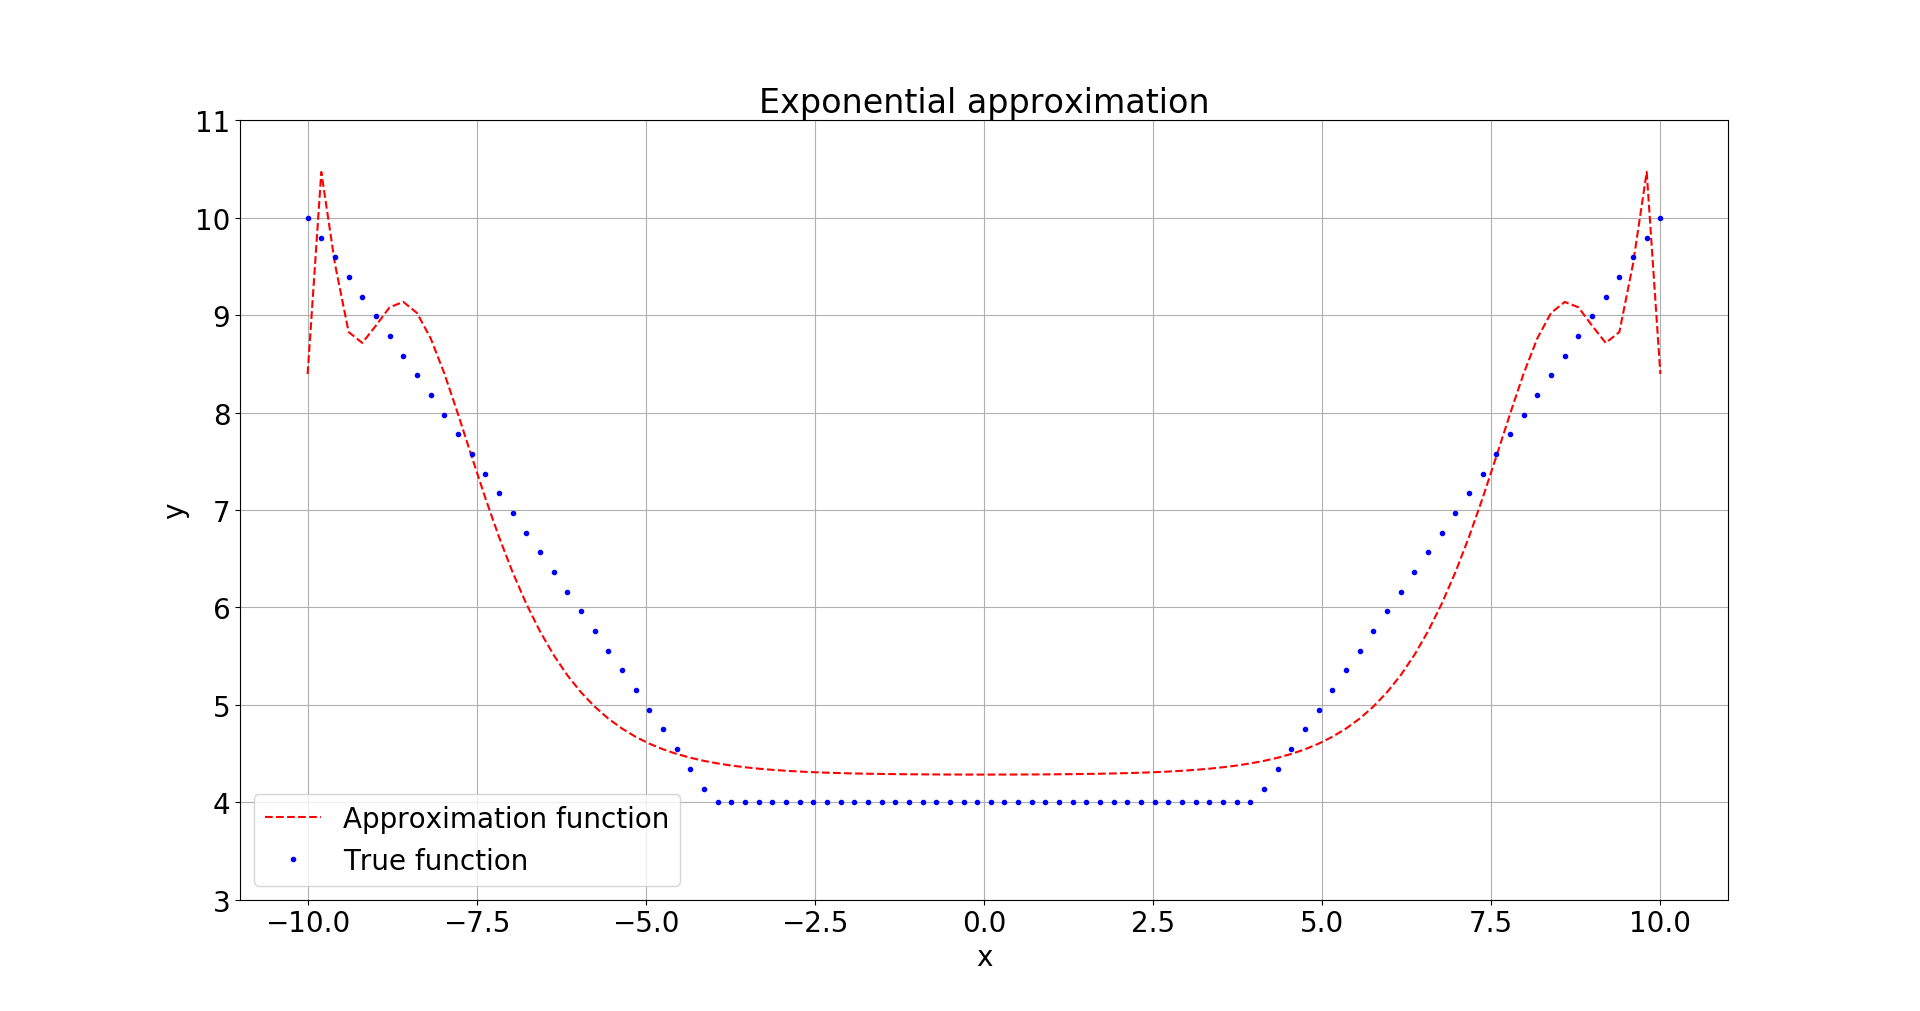
\includegraphics[width=\textwidth]{2.png}
\end{figure}
\[ \Delta^2(f) = \texttt{0.10740063553045082}. \]

% \subsubsection{Експоненційна система функцій}
% \begin{figure}[H]
%     \centering
%     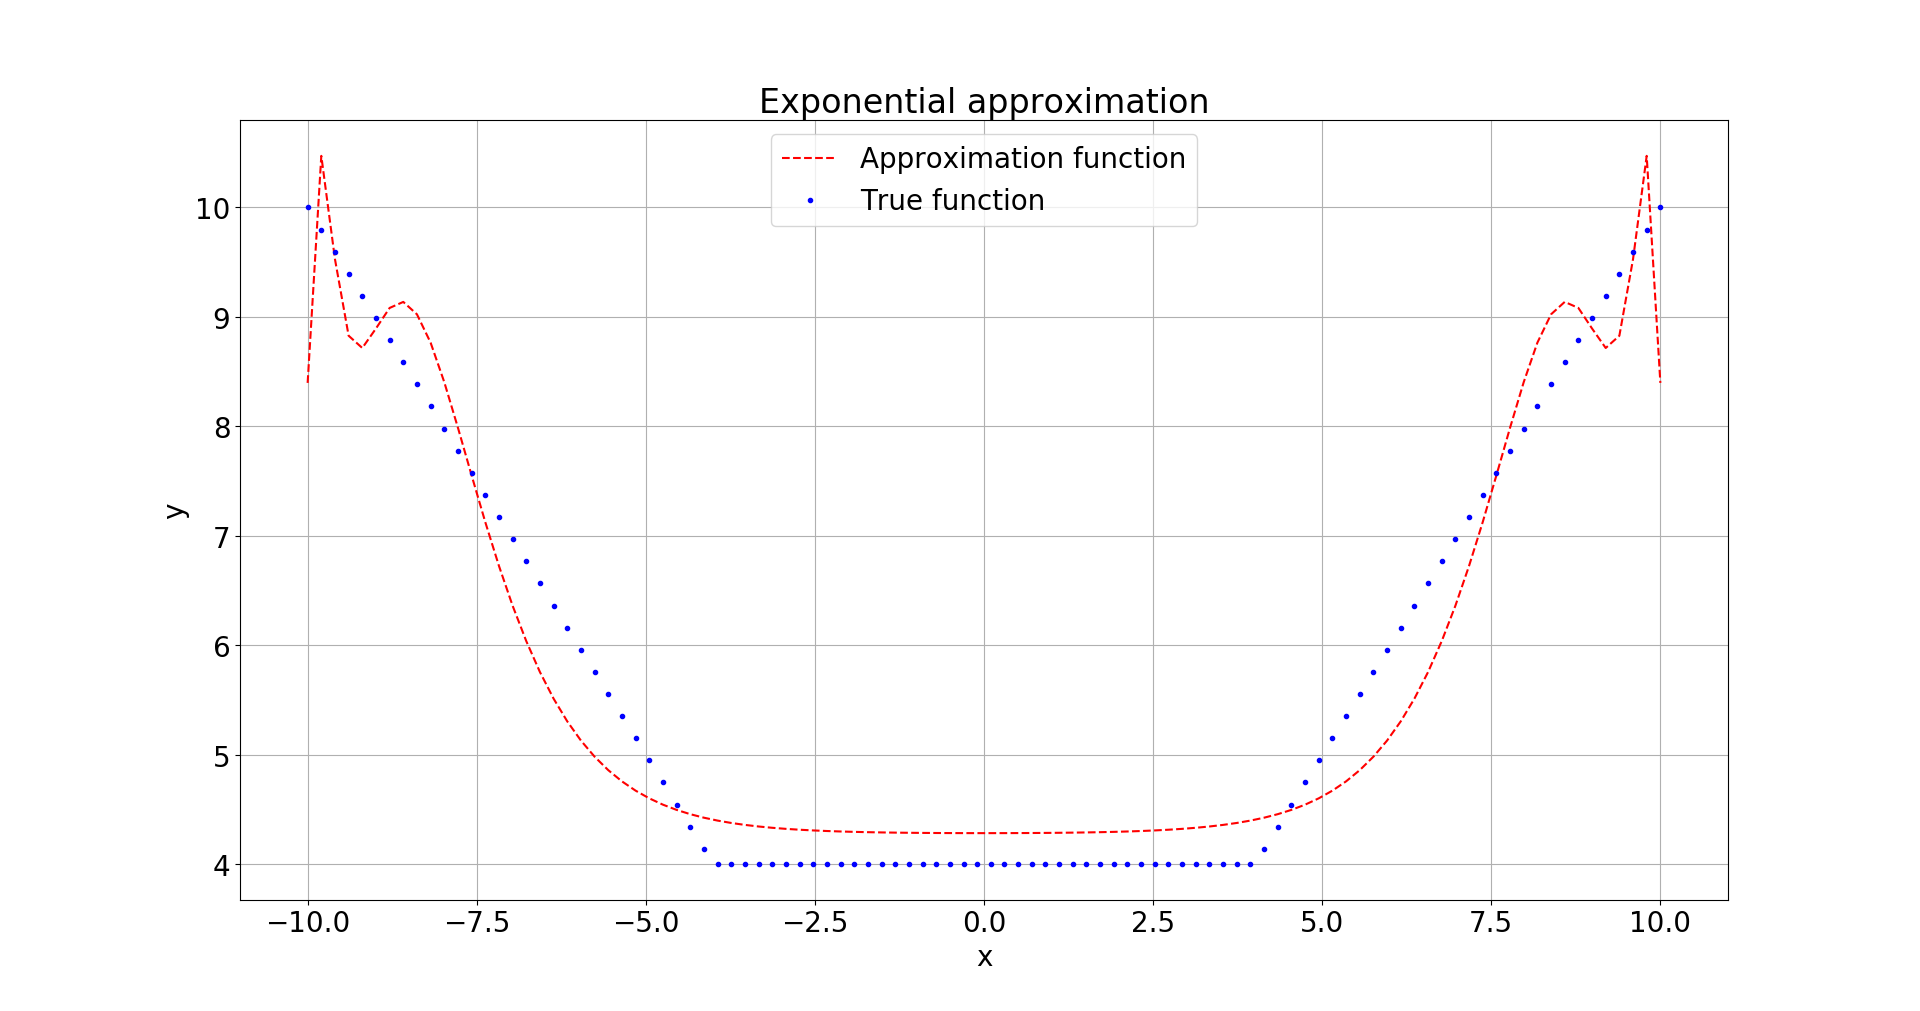
\includegraphics[width=\textwidth]{6.png}
% \end{figure}
% \[ \Delta^2(f) = \texttt{4.20306095641598}. \]


\subsection{Метод найменших квадратів}

Маємо таблицю значень:

\begin{table}[H]
    \centering
    \begin{tabular}{|c|c|c|c|c|c|c|c|c|c|c|} \hline
        $i$ & 0 & 1 & 2 & 3 & 4 & 5 & 6 & 7 & 8 & 9 \\ \hline
        $x_i$ & $-10$ & $-9$ & $-8$ & $-7$ & $-6$ & $-5$ & $-4$ & $-3$ & $-2$ & $-1$ \\ \hline 
        $y_i$ & 10 & 9 & 8 & 7 & 6 & 5 & 4 & 4 & 4 & 4 \\ \hline
    \end{tabular}
    \break
    \hfill 
    \break
    \begin{tabular}{|c|c|c|c|c|c|c|c|c|c|c|c|} \hline
        $i$ & 10 & 11 & 12 & 13 & 14 & 15 & 16 & 17 & 18 & 19 & 20 \\ \hline
        $x_i$ & 0 & 1 & 2 & 3 & 4 & 5 & 6 & 7 & 8 & 9 & 10 \\ \hline
        $y_i$ & 4 & 4 & 4 & 4 & 4 & 5 & 6 & 7 & 8 & 9 & 10 \\ \hline
    \end{tabular}
\end{table}

Знайдемо значення похибки для різних $n$:

\begin{table}[H]
    \tt
    \centering
    \begin{tabular}{|c|c|} \hline
        $n$ & $\sigma_n$ \\ \hline
        1 & 0.2456140350877193000 \\ \hline
        2 & 0.0044225627749655240 \\ \hline
        3 & 0.0046827135264340840 \\ \hline
        4 & 0.0049553959299550940 \\ \hline
        5 & 0.0052857556586187580 \\ \hline
        6 & 0.0024510823676256385 \\ \hline
        7 & 0.0026396271651353076 \\ \hline
        8 & 0.0008506324753000230 \\ \hline
        9 & 0.0009279627003272968 \\ \hline
    \end{tabular}
\end{table}

Як бачимо, стабілізація відбувається починаючи з $n = 2$.

\begin{figure}[H]
    \centering
    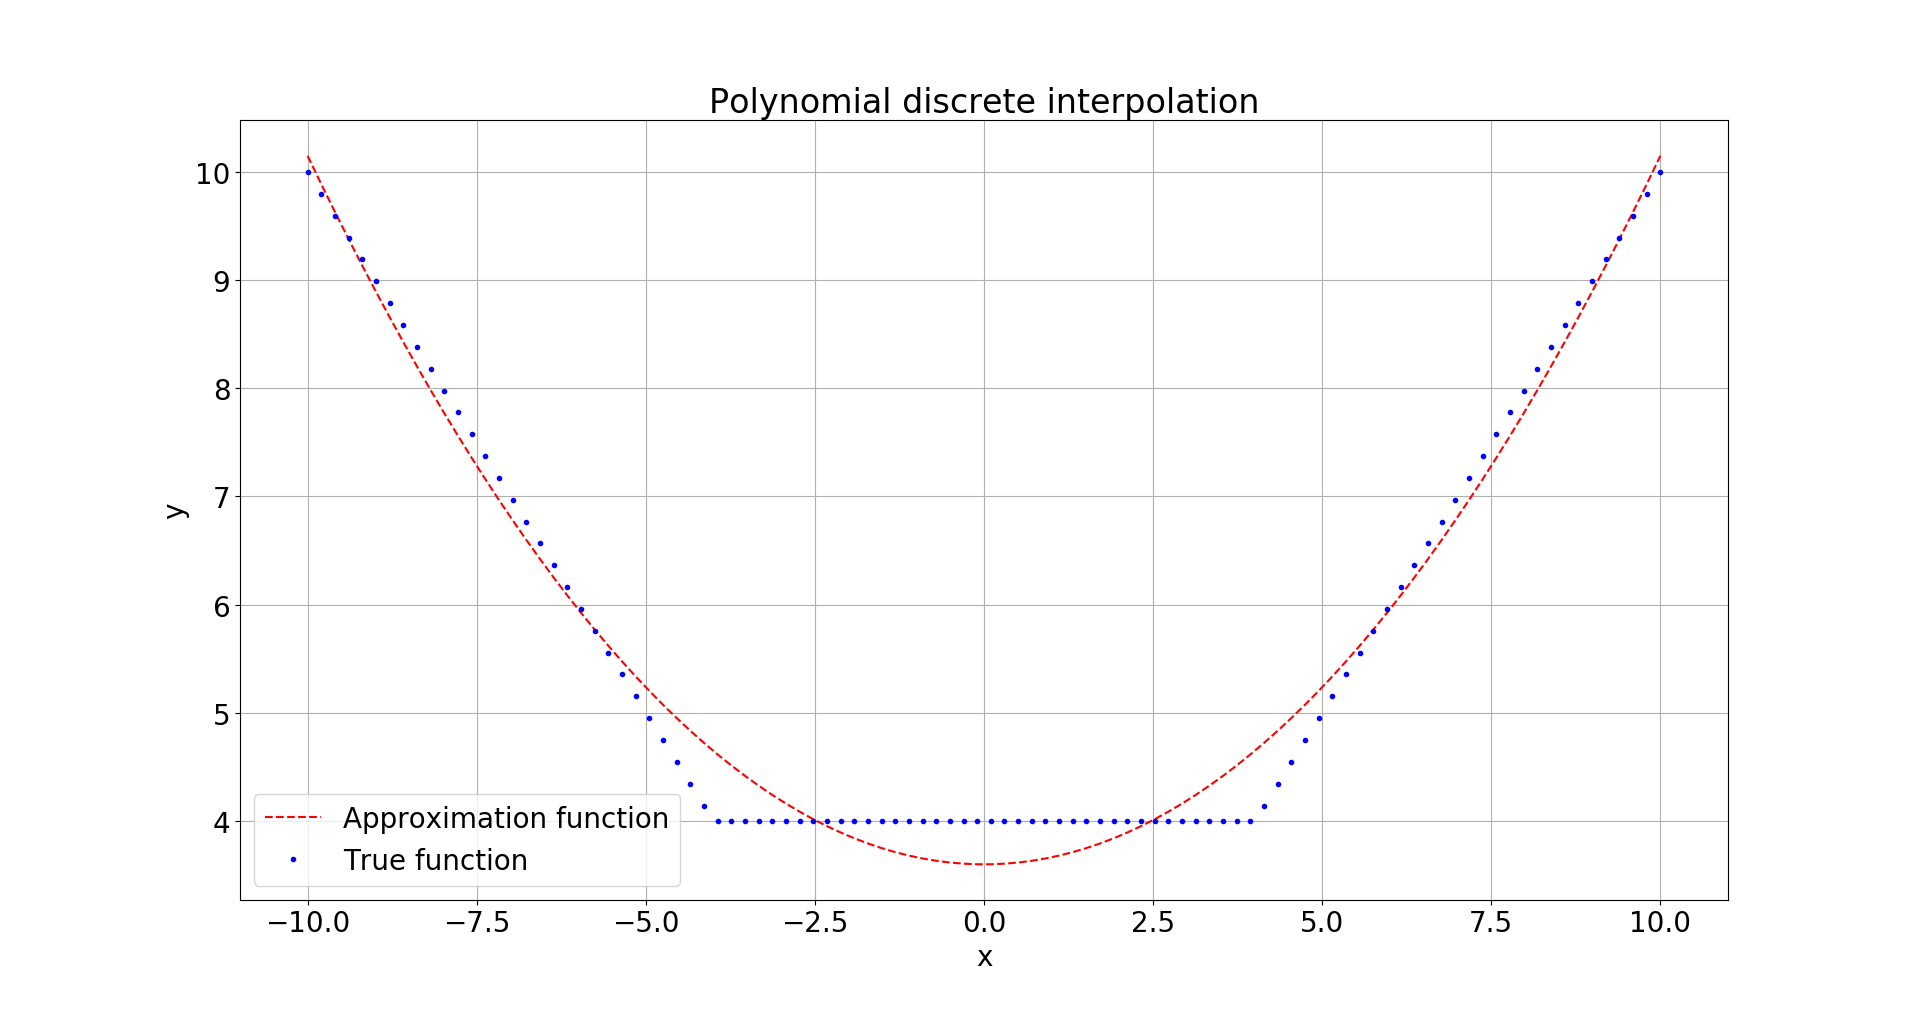
\includegraphics[width=\textwidth]{4.png}
\end{figure}

Відповідна ``похибка'' (у лапках бо взята із ваговим коефіцієнтом): \[ \sigma_2 = \texttt{0.004422562774965524}. \]

\subsection{Кубічні згладжувальні сплайни}

\begin{figure}[H]
    \centering
    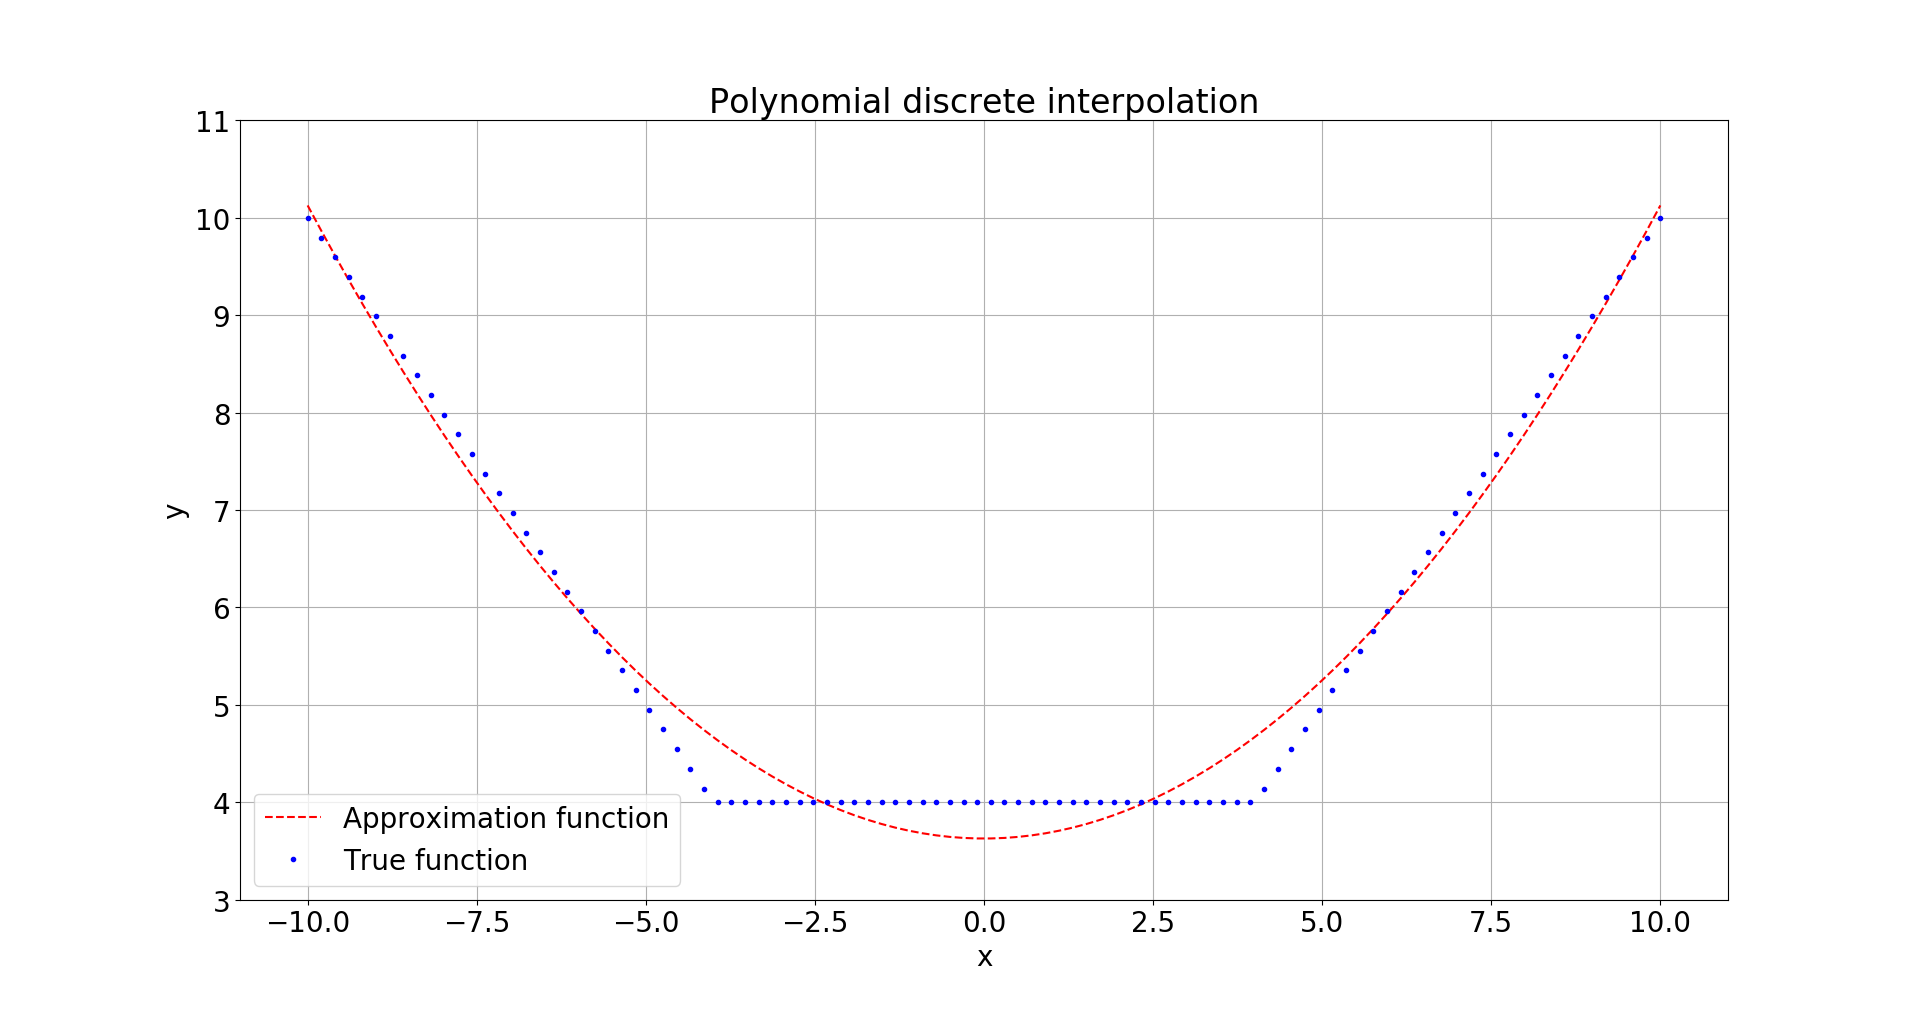
\includegraphics[width=\textwidth]{5.png}
\end{figure}

\end{document}
